% User manual of a V9990 port (homage). Generic body: everything specific to the game is in
%   meta.tex        title, publisher, year, port credits, accent colour, hardware facts
%   lang-LL.tex     the fixed texts in the language LL (en, es)
%   game-LL.tex     the sections about the game (how to play, HUD, scoring, tips)
%   override-LL.tex per-game replacements of the fixed texts (\renewcommand), and
%                   \tCreditsExtra (optional extra \item lines in the credits)
% Build one language:  pdflatex -jobname=manual-LL "\def\manlang{LL}% User manual of a V9990 port (homage). Generic body: everything specific to the game is in
%   meta.tex        title, publisher, year, port credits, accent colour, hardware facts
%   lang-LL.tex     the fixed texts in the language LL (en, es)
%   game-LL.tex     the sections about the game (how to play, HUD, scoring, tips)
%   override-LL.tex per-game replacements of the fixed texts (\renewcommand), and
%                   \tCreditsExtra (optional extra \item lines in the credits)
% Build one language:  pdflatex -jobname=manual-LL "\def\manlang{LL}% User manual of a V9990 port (homage). Generic body: everything specific to the game is in
%   meta.tex        title, publisher, year, port credits, accent colour, hardware facts
%   lang-LL.tex     the fixed texts in the language LL (en, es)
%   game-LL.tex     the sections about the game (how to play, HUD, scoring, tips)
%   override-LL.tex per-game replacements of the fixed texts (\renewcommand), and
%                   \tCreditsExtra (optional extra \item lines in the credits)
% Build one language:  pdflatex -jobname=manual-LL "\def\manlang{LL}% User manual of a V9990 port (homage). Generic body: everything specific to the game is in
%   meta.tex        title, publisher, year, port credits, accent colour, hardware facts
%   lang-LL.tex     the fixed texts in the language LL (en, es)
%   game-LL.tex     the sections about the game (how to play, HUD, scoring, tips)
%   override-LL.tex per-game replacements of the fixed texts (\renewcommand), and
%                   \tCreditsExtra (optional extra \item lines in the credits)
% Build one language:  pdflatex -jobname=manual-LL "\def\manlang{LL}\input{manual}"   (twice)
\documentclass[a4paper,11pt]{article}
\providecommand{\manlang}{en}
\usepackage[utf8]{inputenc}
\usepackage[T1]{fontenc}
\IfFileExists{lmodern.sty}{\usepackage{lmodern}}{}
\usepackage{helvet,longtable}
\renewcommand{\familydefault}{\sfdefault}
\input{meta}
\InputIfFileExists{lang-\manlang}{}{\PackageError{manual}{no lang-\manlang.tex}{}}
\InputIfFileExists{override-\manlang}{}{}   % per-game replacements of the fixed texts
\usepackage[margin=2.2cm,top=2.4cm,bottom=2.4cm]{geometry}
\usepackage{graphicx,xcolor,booktabs,tabularx,float,caption,fancyhdr,eso-pic,parskip,microtype}
\usepackage[hidelinks,pdftitle={\gameTitle{} - \tManual},pdfauthor={\portAuthor}]{hyperref}

\definecolor{accent}{RGB}{\accentRGB}
\definecolor{ink}{RGB}{8,8,20}
\captionsetup{font=small,labelfont=bf}
\setlength{\parindent}{0pt}
\pagestyle{fancy}\fancyhf{}
\fancyhead[L]{\small\textcolor{accent}{\textbf{\MakeUppercase{\gameTitle}}} \tForV}
\fancyhead[R]{\small \tManual}
\fancyfoot[C]{\small\thepage}
\renewcommand{\headrulewidth}{0.4pt}

\newcommand{\key}[1]{{\fboxsep=2.5pt\fbox{\textbf{\strut #1}}}}
\newcommand{\sect}[1]{\section*{\textcolor{accent}{#1}}\addcontentsline{toc}{section}{#1}}
% Keep a reference heading with its table header and first entry.
\newcommand{\refspace}{\par\ifdim\dimexpr\pagegoal-\pagetotal\relax<8\baselineskip\newpage\fi}
% Keep each picture beside its name, including names that wrap to several lines.
\newcommand{\itemname}[2]{%
\begin{minipage}[t]{8mm}\vspace{0pt}\includegraphics[width=7mm]{img/items/#1.png}\end{minipage}%
\hspace{1mm}\begin{minipage}[t]{\dimexpr\linewidth-9mm\relax}\vspace{0pt}\raggedright\textbf{#2}\end{minipage}}
\newcommand{\enemyname}[2]{%
\begin{minipage}[t]{\linewidth}\vspace{0pt}\raggedright
\textbf{#2}\par\smallskip
\includegraphics[width=34mm,height=24mm,keepaspectratio]{img/enemies/#1.png}%
\end{minipage}}
\newenvironment{reference}[2]{\begingroup\small
\renewcommand{\arraystretch}{1.15}
\begin{longtable}{@{}p{0.27\textwidth}p{0.69\textwidth}@{}}
\toprule\textbf{#1}&\textbf{#2}\\\midrule\endfirsthead
\toprule\textbf{#1}&\textbf{#2}\\\midrule\endhead
\bottomrule\endfoot}{\end{longtable}\endgroup}

\begin{document}

% ---------- Cover: the game's cover picture, full page ----------
\thispagestyle{empty}
\AddToShipoutPictureBG*{\put(0,0){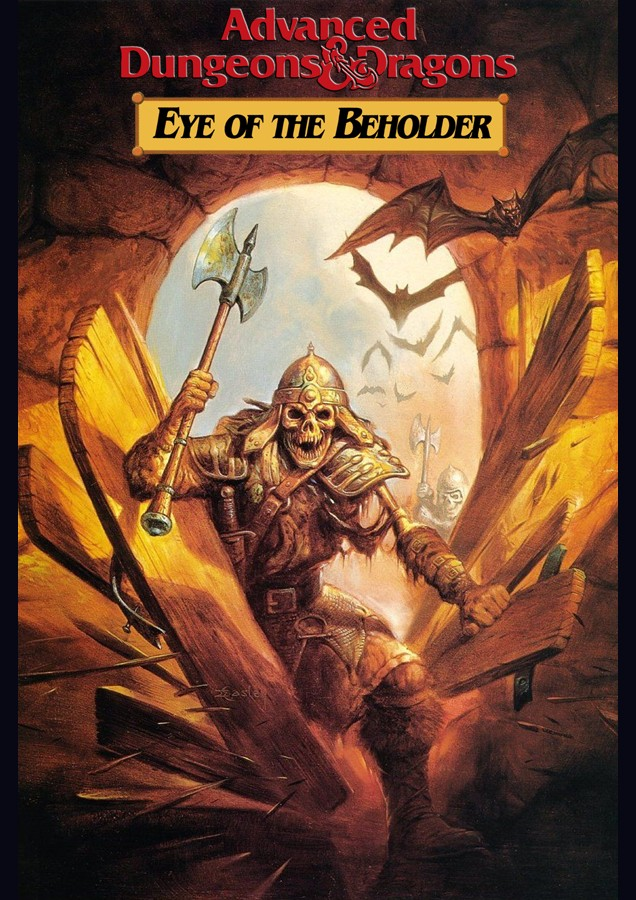
\includegraphics[width=\paperwidth,height=\paperheight]{img/cover.jpg}}%
  \put(0.045\paperwidth,0.108\paperheight){
\includegraphics[width=0.30\paperwidth]{img/msx-logo.png}}%
  \put(0.045\paperwidth,0.05\paperheight){
\includegraphics[width=0.30\paperwidth]{img/v9990-logo.png}}}
\mbox{}\vfill
\begin{flushright}
\colorbox{ink}{\parbox{0.62\textwidth}{\raggedleft\color{white}\vspace{2pt}
{\Large\bfseries \tUserManual}\\[2pt]
{\large \tCoverLine}\vspace{4pt}}}
\end{flushright}
\newpage

% ---------- Title page ----------
\thispagestyle{empty}
\begin{center}
\vspace*{1.2cm}
{\fontsize{34}{38}\selectfont\bfseries\textcolor{accent}{\MakeUppercase{\gameTitle}}}\\[6pt]
{\Large \tForTheV}\\[1.0cm]

\includegraphics[height=2.2cm]{img/msx-logo.png}\hspace{1.2cm}
\includegraphics[height=1.5cm]{img/v9990-logo.png}\\[1.0cm]
\parbox{0.8\textwidth}{\centering
\tOriginalBy{} \textbf{\originalPublisher}, \originalYear.\\[3pt]
\tPortBy{} \textbf{\portAuthor}, \portYear.}\\[1.5cm]
\includegraphics[width=0.8\textwidth]{\imgdir montage.png}
\end{center}
\vfill
{\small \tHomage}
\newpage

\tableofcontents
\newpage

% ==================================================================
\sect{1. \tWhatYouNeed}

\begin{center}
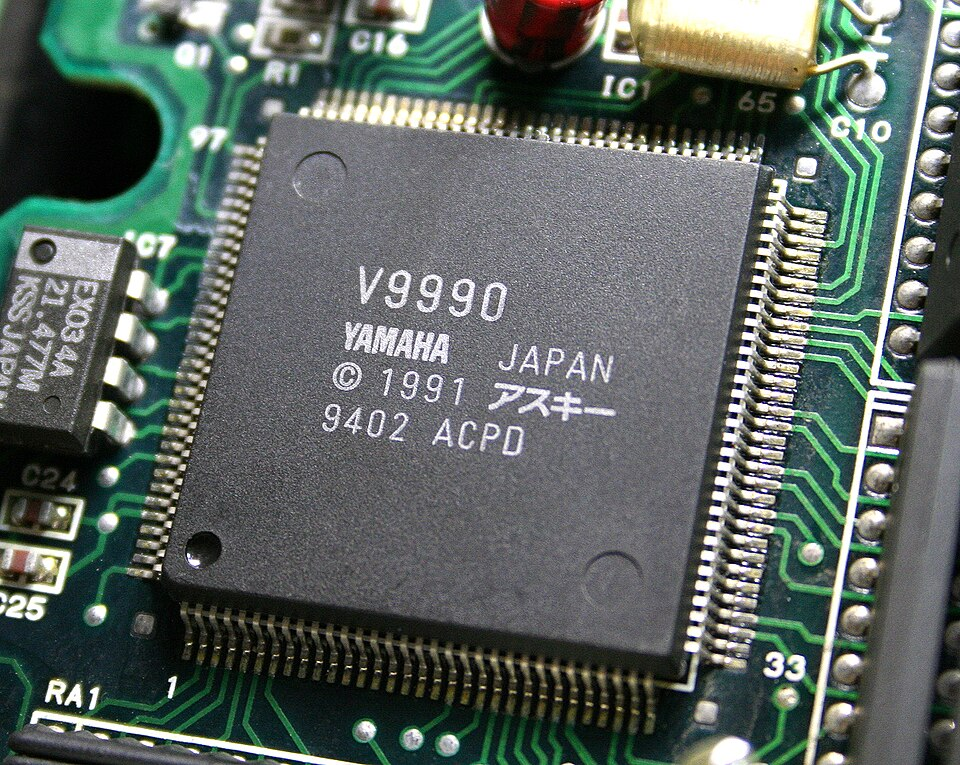
\includegraphics[width=0.62\textwidth]{img/v9990-chip.jpg}
\captionof{figure}{\tChipCaption}
\end{center}

\begin{tabularx}{\textwidth}{@{}lX@{}}
\toprule
\textbf{\tItem} & \textbf{\tRequirement}\\
\midrule
\tComputer & \tComputerText\\
\tMemory & \tMemoryText\\
\tVideo & \tVideoText\\
\tSoundRow & \tSoundText\\
\tGameRow & \tGameText\\
\tMonitor & \tMonitorText\\
\tControlsRow & \tControlsText\\
\bottomrule
\end{tabularx}

\medskip
\tNoTape

% ==================================================================
\sect{2. \tSettingUp}

\begin{enumerate}
\item \tSetOff
\item \tSetV
\item \tSetGame
\item \tSetMonitor
\item \tSetJoy
\item \tSetOn
\end{enumerate}

\tBlackScreen

% ==================================================================
\sect{3. \tPowerOnTitle}

\begin{figure}[H]
\centering
\includegraphics[width=0.48\textwidth]{\imgdir cover-shot.png}\hfill
\includegraphics[width=0.48\textwidth]{\tTitleShot}
\caption{\tPowerOnCaption}
\end{figure}

\input{flow-\manlang}

% ==================================================================
\sect{4. \tControlsTitle}

\input{controls-\manlang}

% ==================================================================
\input{game-\manlang}
\input{bestiary-\manlang}

% ==================================================================
\clearpage
\sect{\tCreditsTitle}

\begin{itemize}
\item \textbf{\gameTitle} \tIsAGameBy{} \textbf{\originalPublisher}, \originalYear. \tRightsText
\item \textbf{\tVersionWord} (\portWork): \textbf{\portAuthor}, \portYear.
\item \tMsxTrademark{} (file \texttt{MSX-Logo.svg}, Wikimedia Commons).
\item \tChipNote
\ifdefined\tCreditsExtra \tCreditsExtra \fi   % optional \item lines (override-LL.tex)
\item \tSourceNote
\end{itemize}

% ==================================================================
% The cartridge label: cartridge games only (\cartridgefalse in meta.tex for
% games on disk, MSX-DOS, hard disk or SD)
\ifcartridge
\newpage
\sect{\tAppendix}

\tStickerText

\begin{center}
\includegraphics[width=\textwidth]{img/sticker.png}
\end{center}
\fi

\end{document}
"   (twice)
\documentclass[a4paper,11pt]{article}
\providecommand{\manlang}{en}
\usepackage[utf8]{inputenc}
\usepackage[T1]{fontenc}
\IfFileExists{lmodern.sty}{\usepackage{lmodern}}{}
\usepackage{helvet,longtable}
\renewcommand{\familydefault}{\sfdefault}
% Facts about the game. Edit this file; manual.tex and the lang files read it.
\newcommand{\gameTitle}{Eye of the Beholder}
\newcommand{\originalPublisher}{Westwood Associates / SSI}
\newcommand{\originalYear}{1991}
\newcommand{\portAuthor}{DiHalt Studio}
\newcommand{\portYear}{2026}
\newcommand{\accentRGB}{175,35,30}      % accent colour of headings (R,G,B), the red of the box title
\newcommand{\romFile}{EOB.COM}          % the program (the game is on disk, not in a cartridge)
\newcommand{\romKind}{MSX-DOS2 / Nextor}
\newcommand{\ramNeeded}{512~KB}
\newcommand{\portWork}{port to MSX-DOS2 with V9990 graphics}
\newcommand{\portWorkES}{adaptación a MSX-DOS2 con gráficos para V9990}
% A game on disk (MSX-DOS2 / Nextor, hard disk or SD): no cartridge label.
\newif\ifcartridge
\cartridgefalse

\InputIfFileExists{lang-\manlang}{}{\PackageError{manual}{no lang-\manlang.tex}{}}
\InputIfFileExists{override-\manlang}{}{}   % per-game replacements of the fixed texts
\usepackage[margin=2.2cm,top=2.4cm,bottom=2.4cm]{geometry}
\usepackage{graphicx,xcolor,booktabs,tabularx,float,caption,fancyhdr,eso-pic,parskip,microtype}
\usepackage[hidelinks,pdftitle={\gameTitle{} - \tManual},pdfauthor={\portAuthor}]{hyperref}

\definecolor{accent}{RGB}{\accentRGB}
\definecolor{ink}{RGB}{8,8,20}
\captionsetup{font=small,labelfont=bf}
\setlength{\parindent}{0pt}
\pagestyle{fancy}\fancyhf{}
\fancyhead[L]{\small\textcolor{accent}{\textbf{\MakeUppercase{\gameTitle}}} \tForV}
\fancyhead[R]{\small \tManual}
\fancyfoot[C]{\small\thepage}
\renewcommand{\headrulewidth}{0.4pt}

\newcommand{\key}[1]{{\fboxsep=2.5pt\fbox{\textbf{\strut #1}}}}
\newcommand{\sect}[1]{\section*{\textcolor{accent}{#1}}\addcontentsline{toc}{section}{#1}}
% Keep a reference heading with its table header and first entry.
\newcommand{\refspace}{\par\ifdim\dimexpr\pagegoal-\pagetotal\relax<8\baselineskip\newpage\fi}
% Keep each picture beside its name, including names that wrap to several lines.
\newcommand{\itemname}[2]{%
\begin{minipage}[t]{8mm}\vspace{0pt}\includegraphics[width=7mm]{img/items/#1.png}\end{minipage}%
\hspace{1mm}\begin{minipage}[t]{\dimexpr\linewidth-9mm\relax}\vspace{0pt}\raggedright\textbf{#2}\end{minipage}}
\newcommand{\enemyname}[2]{%
\begin{minipage}[t]{\linewidth}\vspace{0pt}\raggedright
\textbf{#2}\par\smallskip
\includegraphics[width=34mm,height=24mm,keepaspectratio]{img/enemies/#1.png}%
\end{minipage}}
\newenvironment{reference}[2]{\begingroup\small
\renewcommand{\arraystretch}{1.15}
\begin{longtable}{@{}p{0.27\textwidth}p{0.69\textwidth}@{}}
\toprule\textbf{#1}&\textbf{#2}\\\midrule\endfirsthead
\toprule\textbf{#1}&\textbf{#2}\\\midrule\endhead
\bottomrule\endfoot}{\end{longtable}\endgroup}

\begin{document}

% ---------- Cover: the game's cover picture, full page ----------
\thispagestyle{empty}
\AddToShipoutPictureBG*{\put(0,0){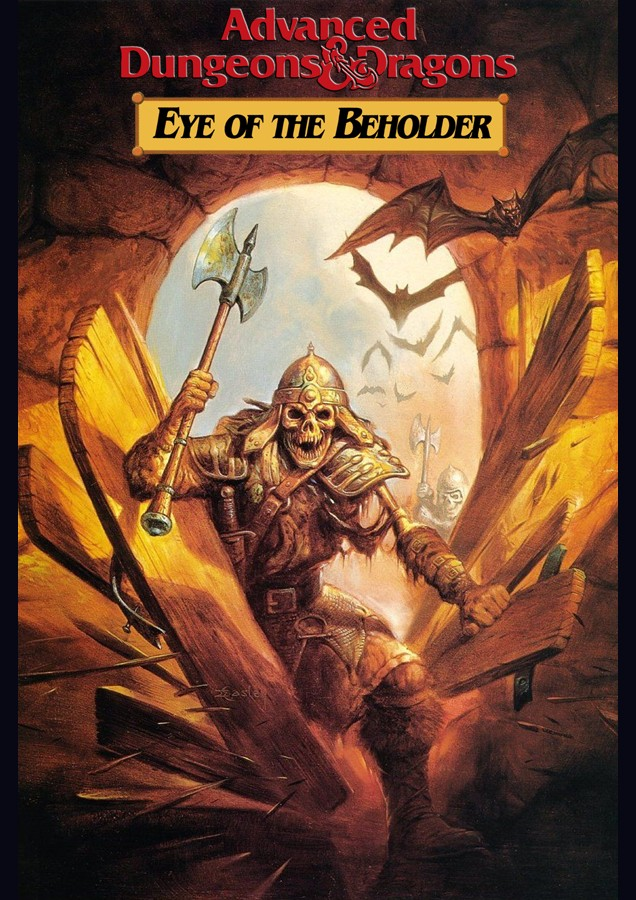
\includegraphics[width=\paperwidth,height=\paperheight]{img/cover.jpg}}%
  \put(0.045\paperwidth,0.108\paperheight){
\includegraphics[width=0.30\paperwidth]{img/msx-logo.png}}%
  \put(0.045\paperwidth,0.05\paperheight){
\includegraphics[width=0.30\paperwidth]{img/v9990-logo.png}}}
\mbox{}\vfill
\begin{flushright}
\colorbox{ink}{\parbox{0.62\textwidth}{\raggedleft\color{white}\vspace{2pt}
{\Large\bfseries \tUserManual}\\[2pt]
{\large \tCoverLine}\vspace{4pt}}}
\end{flushright}
\newpage

% ---------- Title page ----------
\thispagestyle{empty}
\begin{center}
\vspace*{1.2cm}
{\fontsize{34}{38}\selectfont\bfseries\textcolor{accent}{\MakeUppercase{\gameTitle}}}\\[6pt]
{\Large \tForTheV}\\[1.0cm]

\includegraphics[height=2.2cm]{img/msx-logo.png}\hspace{1.2cm}
\includegraphics[height=1.5cm]{img/v9990-logo.png}\\[1.0cm]
\parbox{0.8\textwidth}{\centering
\tOriginalBy{} \textbf{\originalPublisher}, \originalYear.\\[3pt]
\tPortBy{} \textbf{\portAuthor}, \portYear.}\\[1.5cm]
\includegraphics[width=0.8\textwidth]{\imgdir montage.png}
\end{center}
\vfill
{\small \tHomage}
\newpage

\tableofcontents
\newpage

% ==================================================================
\sect{1. \tWhatYouNeed}

\begin{center}
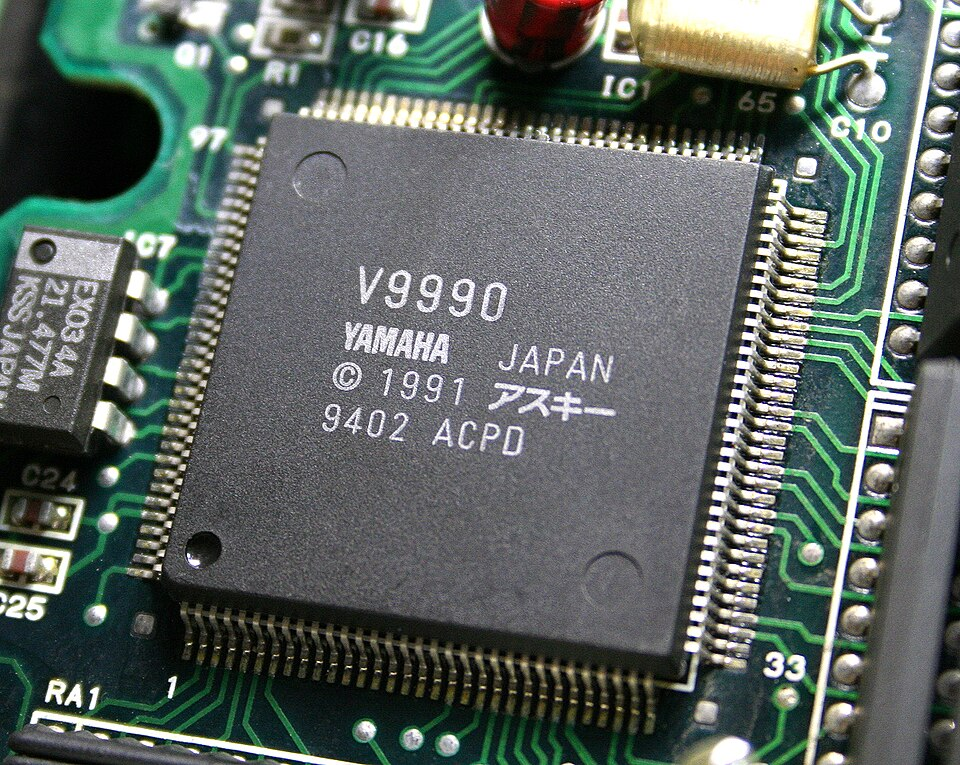
\includegraphics[width=0.62\textwidth]{img/v9990-chip.jpg}
\captionof{figure}{\tChipCaption}
\end{center}

\begin{tabularx}{\textwidth}{@{}lX@{}}
\toprule
\textbf{\tItem} & \textbf{\tRequirement}\\
\midrule
\tComputer & \tComputerText\\
\tMemory & \tMemoryText\\
\tVideo & \tVideoText\\
\tSoundRow & \tSoundText\\
\tGameRow & \tGameText\\
\tMonitor & \tMonitorText\\
\tControlsRow & \tControlsText\\
\bottomrule
\end{tabularx}

\medskip
\tNoTape

% ==================================================================
\sect{2. \tSettingUp}

\begin{enumerate}
\item \tSetOff
\item \tSetV
\item \tSetGame
\item \tSetMonitor
\item \tSetJoy
\item \tSetOn
\end{enumerate}

\tBlackScreen

% ==================================================================
\sect{3. \tPowerOnTitle}

\begin{figure}[H]
\centering
\includegraphics[width=0.48\textwidth]{\imgdir cover-shot.png}\hfill
\includegraphics[width=0.48\textwidth]{\tTitleShot}
\caption{\tPowerOnCaption}
\end{figure}

\input{flow-\manlang}

% ==================================================================
\sect{4. \tControlsTitle}

\input{controls-\manlang}

% ==================================================================
\input{game-\manlang}
\input{bestiary-\manlang}

% ==================================================================
\clearpage
\sect{\tCreditsTitle}

\begin{itemize}
\item \textbf{\gameTitle} \tIsAGameBy{} \textbf{\originalPublisher}, \originalYear. \tRightsText
\item \textbf{\tVersionWord} (\portWork): \textbf{\portAuthor}, \portYear.
\item \tMsxTrademark{} (file \texttt{MSX-Logo.svg}, Wikimedia Commons).
\item \tChipNote
\ifdefined\tCreditsExtra \tCreditsExtra \fi   % optional \item lines (override-LL.tex)
\item \tSourceNote
\end{itemize}

% ==================================================================
% The cartridge label: cartridge games only (\cartridgefalse in meta.tex for
% games on disk, MSX-DOS, hard disk or SD)
\ifcartridge
\newpage
\sect{\tAppendix}

\tStickerText

\begin{center}
\includegraphics[width=\textwidth]{img/sticker.png}
\end{center}
\fi

\end{document}
"   (twice)
\documentclass[a4paper,11pt]{article}
\providecommand{\manlang}{en}
\usepackage[utf8]{inputenc}
\usepackage[T1]{fontenc}
\IfFileExists{lmodern.sty}{\usepackage{lmodern}}{}
\usepackage{helvet,longtable}
\renewcommand{\familydefault}{\sfdefault}
% Facts about the game. Edit this file; manual.tex and the lang files read it.
\newcommand{\gameTitle}{Eye of the Beholder}
\newcommand{\originalPublisher}{Westwood Associates / SSI}
\newcommand{\originalYear}{1991}
\newcommand{\portAuthor}{DiHalt Studio}
\newcommand{\portYear}{2026}
\newcommand{\accentRGB}{175,35,30}      % accent colour of headings (R,G,B), the red of the box title
\newcommand{\romFile}{EOB.COM}          % the program (the game is on disk, not in a cartridge)
\newcommand{\romKind}{MSX-DOS2 / Nextor}
\newcommand{\ramNeeded}{512~KB}
\newcommand{\portWork}{port to MSX-DOS2 with V9990 graphics}
\newcommand{\portWorkES}{adaptación a MSX-DOS2 con gráficos para V9990}
% A game on disk (MSX-DOS2 / Nextor, hard disk or SD): no cartridge label.
\newif\ifcartridge
\cartridgefalse

\InputIfFileExists{lang-\manlang}{}{\PackageError{manual}{no lang-\manlang.tex}{}}
\InputIfFileExists{override-\manlang}{}{}   % per-game replacements of the fixed texts
\usepackage[margin=2.2cm,top=2.4cm,bottom=2.4cm]{geometry}
\usepackage{graphicx,xcolor,booktabs,tabularx,float,caption,fancyhdr,eso-pic,parskip,microtype}
\usepackage[hidelinks,pdftitle={\gameTitle{} - \tManual},pdfauthor={\portAuthor}]{hyperref}

\definecolor{accent}{RGB}{\accentRGB}
\definecolor{ink}{RGB}{8,8,20}
\captionsetup{font=small,labelfont=bf}
\setlength{\parindent}{0pt}
\pagestyle{fancy}\fancyhf{}
\fancyhead[L]{\small\textcolor{accent}{\textbf{\MakeUppercase{\gameTitle}}} \tForV}
\fancyhead[R]{\small \tManual}
\fancyfoot[C]{\small\thepage}
\renewcommand{\headrulewidth}{0.4pt}

\newcommand{\key}[1]{{\fboxsep=2.5pt\fbox{\textbf{\strut #1}}}}
\newcommand{\sect}[1]{\section*{\textcolor{accent}{#1}}\addcontentsline{toc}{section}{#1}}
% Keep a reference heading with its table header and first entry.
\newcommand{\refspace}{\par\ifdim\dimexpr\pagegoal-\pagetotal\relax<8\baselineskip\newpage\fi}
% Keep each picture beside its name, including names that wrap to several lines.
\newcommand{\itemname}[2]{%
\begin{minipage}[t]{8mm}\vspace{0pt}\includegraphics[width=7mm]{img/items/#1.png}\end{minipage}%
\hspace{1mm}\begin{minipage}[t]{\dimexpr\linewidth-9mm\relax}\vspace{0pt}\raggedright\textbf{#2}\end{minipage}}
\newcommand{\enemyname}[2]{%
\begin{minipage}[t]{\linewidth}\vspace{0pt}\raggedright
\textbf{#2}\par\smallskip
\includegraphics[width=34mm,height=24mm,keepaspectratio]{img/enemies/#1.png}%
\end{minipage}}
\newenvironment{reference}[2]{\begingroup\small
\renewcommand{\arraystretch}{1.15}
\begin{longtable}{@{}p{0.27\textwidth}p{0.69\textwidth}@{}}
\toprule\textbf{#1}&\textbf{#2}\\\midrule\endfirsthead
\toprule\textbf{#1}&\textbf{#2}\\\midrule\endhead
\bottomrule\endfoot}{\end{longtable}\endgroup}

\begin{document}

% ---------- Cover: the game's cover picture, full page ----------
\thispagestyle{empty}
\AddToShipoutPictureBG*{\put(0,0){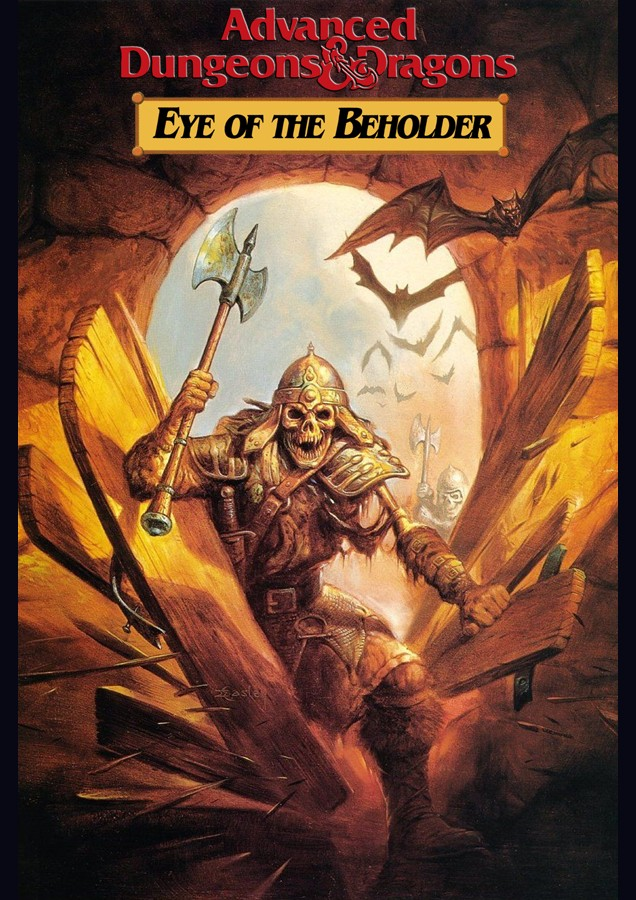
\includegraphics[width=\paperwidth,height=\paperheight]{img/cover.jpg}}%
  \put(0.045\paperwidth,0.108\paperheight){
\includegraphics[width=0.30\paperwidth]{img/msx-logo.png}}%
  \put(0.045\paperwidth,0.05\paperheight){
\includegraphics[width=0.30\paperwidth]{img/v9990-logo.png}}}
\mbox{}\vfill
\begin{flushright}
\colorbox{ink}{\parbox{0.62\textwidth}{\raggedleft\color{white}\vspace{2pt}
{\Large\bfseries \tUserManual}\\[2pt]
{\large \tCoverLine}\vspace{4pt}}}
\end{flushright}
\newpage

% ---------- Title page ----------
\thispagestyle{empty}
\begin{center}
\vspace*{1.2cm}
{\fontsize{34}{38}\selectfont\bfseries\textcolor{accent}{\MakeUppercase{\gameTitle}}}\\[6pt]
{\Large \tForTheV}\\[1.0cm]

\includegraphics[height=2.2cm]{img/msx-logo.png}\hspace{1.2cm}
\includegraphics[height=1.5cm]{img/v9990-logo.png}\\[1.0cm]
\parbox{0.8\textwidth}{\centering
\tOriginalBy{} \textbf{\originalPublisher}, \originalYear.\\[3pt]
\tPortBy{} \textbf{\portAuthor}, \portYear.}\\[1.5cm]
\includegraphics[width=0.8\textwidth]{\imgdir montage.png}
\end{center}
\vfill
{\small \tHomage}
\newpage

\tableofcontents
\newpage

% ==================================================================
\sect{1. \tWhatYouNeed}

\begin{center}
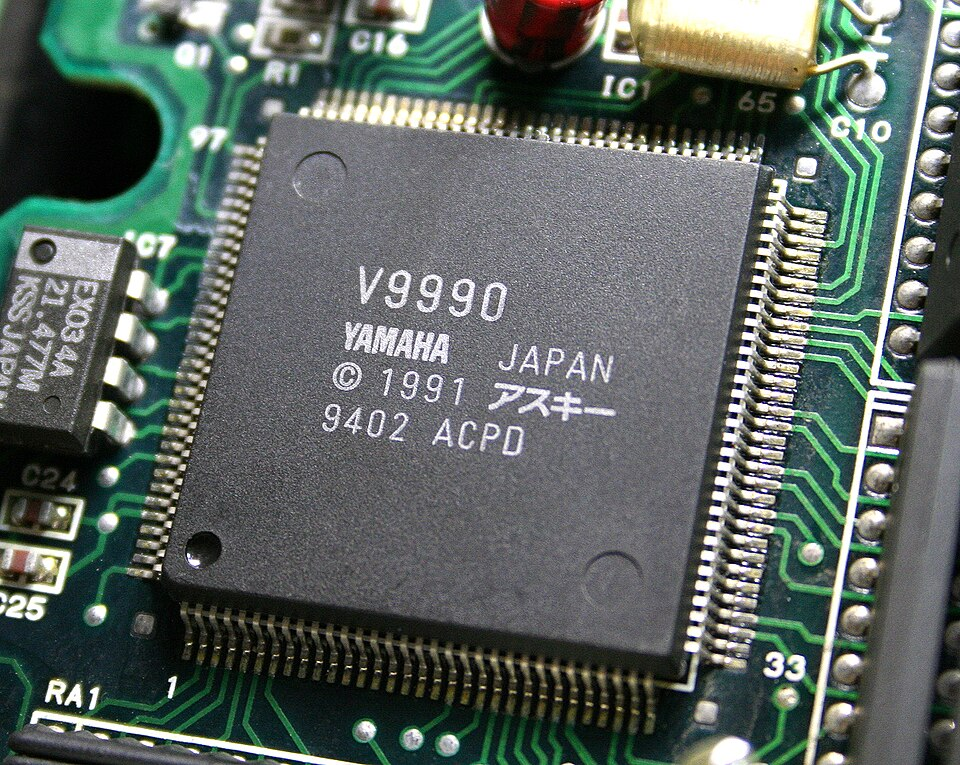
\includegraphics[width=0.62\textwidth]{img/v9990-chip.jpg}
\captionof{figure}{\tChipCaption}
\end{center}

\begin{tabularx}{\textwidth}{@{}lX@{}}
\toprule
\textbf{\tItem} & \textbf{\tRequirement}\\
\midrule
\tComputer & \tComputerText\\
\tMemory & \tMemoryText\\
\tVideo & \tVideoText\\
\tSoundRow & \tSoundText\\
\tGameRow & \tGameText\\
\tMonitor & \tMonitorText\\
\tControlsRow & \tControlsText\\
\bottomrule
\end{tabularx}

\medskip
\tNoTape

% ==================================================================
\sect{2. \tSettingUp}

\begin{enumerate}
\item \tSetOff
\item \tSetV
\item \tSetGame
\item \tSetMonitor
\item \tSetJoy
\item \tSetOn
\end{enumerate}

\tBlackScreen

% ==================================================================
\sect{3. \tPowerOnTitle}

\begin{figure}[H]
\centering
\includegraphics[width=0.48\textwidth]{\imgdir cover-shot.png}\hfill
\includegraphics[width=0.48\textwidth]{\tTitleShot}
\caption{\tPowerOnCaption}
\end{figure}

\input{flow-\manlang}

% ==================================================================
\sect{4. \tControlsTitle}

\input{controls-\manlang}

% ==================================================================
\input{game-\manlang}
\input{bestiary-\manlang}

% ==================================================================
\clearpage
\sect{\tCreditsTitle}

\begin{itemize}
\item \textbf{\gameTitle} \tIsAGameBy{} \textbf{\originalPublisher}, \originalYear. \tRightsText
\item \textbf{\tVersionWord} (\portWork): \textbf{\portAuthor}, \portYear.
\item \tMsxTrademark{} (file \texttt{MSX-Logo.svg}, Wikimedia Commons).
\item \tChipNote
\ifdefined\tCreditsExtra \tCreditsExtra \fi   % optional \item lines (override-LL.tex)
\item \tSourceNote
\end{itemize}

% ==================================================================
% The cartridge label: cartridge games only (\cartridgefalse in meta.tex for
% games on disk, MSX-DOS, hard disk or SD)
\ifcartridge
\newpage
\sect{\tAppendix}

\tStickerText

\begin{center}
\includegraphics[width=\textwidth]{img/sticker.png}
\end{center}
\fi

\end{document}
"   (twice)
\documentclass[a4paper,11pt]{article}
\providecommand{\manlang}{en}
\usepackage[utf8]{inputenc}
\usepackage[T1]{fontenc}
\IfFileExists{lmodern.sty}{\usepackage{lmodern}}{}
\usepackage{helvet,longtable}
\renewcommand{\familydefault}{\sfdefault}
% Facts about the game. Edit this file; manual.tex and the lang files read it.
\newcommand{\gameTitle}{Eye of the Beholder}
\newcommand{\originalPublisher}{Westwood Associates / SSI}
\newcommand{\originalYear}{1991}
\newcommand{\portAuthor}{DiHalt Studio}
\newcommand{\portYear}{2026}
\newcommand{\accentRGB}{175,35,30}      % accent colour of headings (R,G,B), the red of the box title
\newcommand{\romFile}{EOB.COM}          % the program (the game is on disk, not in a cartridge)
\newcommand{\romKind}{MSX-DOS2 / Nextor}
\newcommand{\ramNeeded}{512~KB}
\newcommand{\portWork}{port to MSX-DOS2 with V9990 graphics}
\newcommand{\portWorkES}{adaptación a MSX-DOS2 con gráficos para V9990}
% A game on disk (MSX-DOS2 / Nextor, hard disk or SD): no cartridge label.
\newif\ifcartridge
\cartridgefalse

\InputIfFileExists{lang-\manlang}{}{\PackageError{manual}{no lang-\manlang.tex}{}}
\InputIfFileExists{override-\manlang}{}{}   % per-game replacements of the fixed texts
\usepackage[margin=2.2cm,top=2.4cm,bottom=2.4cm]{geometry}
\usepackage{graphicx,xcolor,booktabs,tabularx,float,caption,fancyhdr,eso-pic,parskip,microtype}
\usepackage[hidelinks,pdftitle={\gameTitle{} - \tManual},pdfauthor={\portAuthor}]{hyperref}

\definecolor{accent}{RGB}{\accentRGB}
\definecolor{ink}{RGB}{8,8,20}
\captionsetup{font=small,labelfont=bf}
\setlength{\parindent}{0pt}
\pagestyle{fancy}\fancyhf{}
\fancyhead[L]{\small\textcolor{accent}{\textbf{\MakeUppercase{\gameTitle}}} \tForV}
\fancyhead[R]{\small \tManual}
\fancyfoot[C]{\small\thepage}
\renewcommand{\headrulewidth}{0.4pt}

\newcommand{\key}[1]{{\fboxsep=2.5pt\fbox{\textbf{\strut #1}}}}
\newcommand{\sect}[1]{\section*{\textcolor{accent}{#1}}\addcontentsline{toc}{section}{#1}}
% Keep a reference heading with its table header and first entry.
\newcommand{\refspace}{\par\ifdim\dimexpr\pagegoal-\pagetotal\relax<8\baselineskip\newpage\fi}
% Keep each picture beside its name, including names that wrap to several lines.
\newcommand{\itemname}[2]{%
\begin{minipage}[t]{8mm}\vspace{0pt}\includegraphics[width=7mm]{img/items/#1.png}\end{minipage}%
\hspace{1mm}\begin{minipage}[t]{\dimexpr\linewidth-9mm\relax}\vspace{0pt}\raggedright\textbf{#2}\end{minipage}}
\newcommand{\enemyname}[2]{%
\begin{minipage}[t]{\linewidth}\vspace{0pt}\raggedright
\textbf{#2}\par\smallskip
\includegraphics[width=34mm,height=24mm,keepaspectratio]{img/enemies/#1.png}%
\end{minipage}}
\newenvironment{reference}[2]{\begingroup\small
\renewcommand{\arraystretch}{1.15}
\begin{longtable}{@{}p{0.27\textwidth}p{0.69\textwidth}@{}}
\toprule\textbf{#1}&\textbf{#2}\\\midrule\endfirsthead
\toprule\textbf{#1}&\textbf{#2}\\\midrule\endhead
\bottomrule\endfoot}{\end{longtable}\endgroup}

\begin{document}

% ---------- Cover: the game's cover picture, full page ----------
\thispagestyle{empty}
\AddToShipoutPictureBG*{\put(0,0){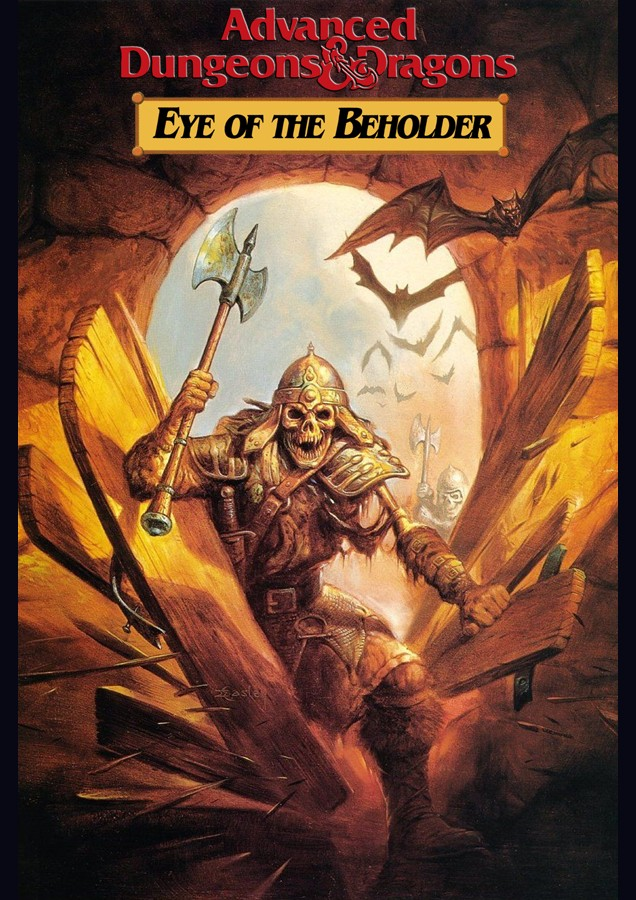
\includegraphics[width=\paperwidth,height=\paperheight]{img/cover.jpg}}%
  \put(0.045\paperwidth,0.108\paperheight){
\includegraphics[width=0.30\paperwidth]{img/msx-logo.png}}%
  \put(0.045\paperwidth,0.05\paperheight){
\includegraphics[width=0.30\paperwidth]{img/v9990-logo.png}}}
\mbox{}\vfill
\begin{flushright}
\colorbox{ink}{\parbox{0.62\textwidth}{\raggedleft\color{white}\vspace{2pt}
{\Large\bfseries \tUserManual}\\[2pt]
{\large \tCoverLine}\vspace{4pt}}}
\end{flushright}
\newpage

% ---------- Title page ----------
\thispagestyle{empty}
\begin{center}
\vspace*{1.2cm}
{\fontsize{34}{38}\selectfont\bfseries\textcolor{accent}{\MakeUppercase{\gameTitle}}}\\[6pt]
{\Large \tForTheV}\\[1.0cm]

\includegraphics[height=2.2cm]{img/msx-logo.png}\hspace{1.2cm}
\includegraphics[height=1.5cm]{img/v9990-logo.png}\\[1.0cm]
\parbox{0.8\textwidth}{\centering
\tOriginalBy{} \textbf{\originalPublisher}, \originalYear.\\[3pt]
\tPortBy{} \textbf{\portAuthor}, \portYear.}\\[1.5cm]
\includegraphics[width=0.8\textwidth]{\imgdir montage.png}
\end{center}
\vfill
{\small \tHomage}
\newpage

\tableofcontents
\newpage

% ==================================================================
\sect{1. \tWhatYouNeed}

\begin{center}
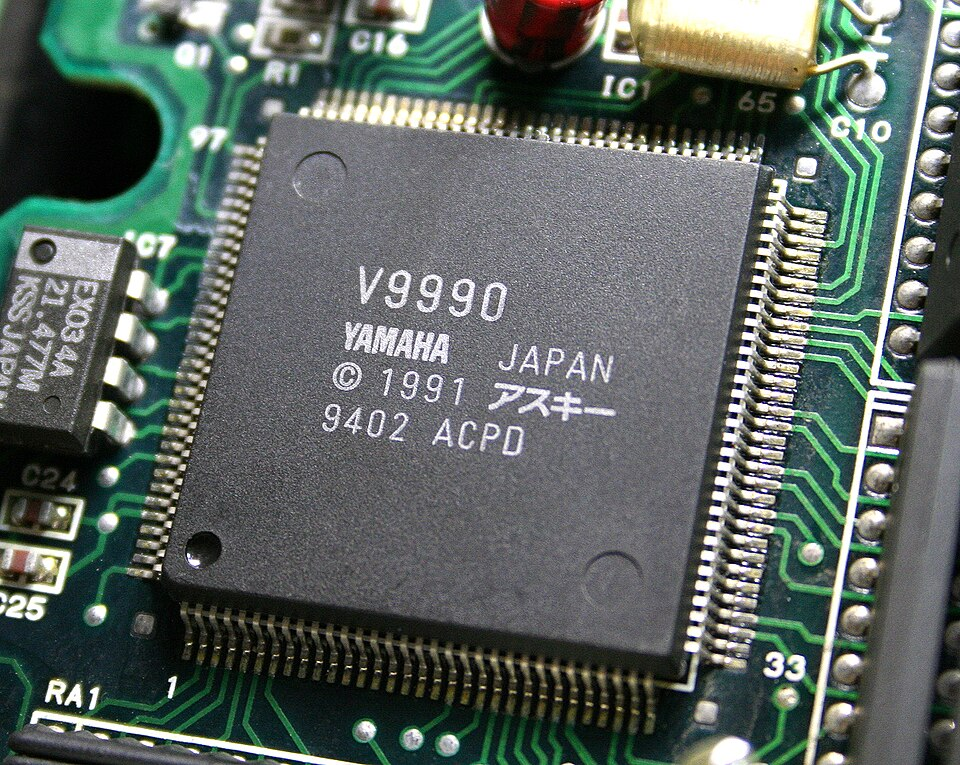
\includegraphics[width=0.62\textwidth]{img/v9990-chip.jpg}
\captionof{figure}{\tChipCaption}
\end{center}

\begin{tabularx}{\textwidth}{@{}lX@{}}
\toprule
\textbf{\tItem} & \textbf{\tRequirement}\\
\midrule
\tComputer & \tComputerText\\
\tMemory & \tMemoryText\\
\tVideo & \tVideoText\\
\tSoundRow & \tSoundText\\
\tGameRow & \tGameText\\
\tMonitor & \tMonitorText\\
\tControlsRow & \tControlsText\\
\bottomrule
\end{tabularx}

\medskip
\tNoTape

% ==================================================================
\sect{2. \tSettingUp}

\begin{enumerate}
\item \tSetOff
\item \tSetV
\item \tSetGame
\item \tSetMonitor
\item \tSetJoy
\item \tSetOn
\end{enumerate}

\tBlackScreen

% ==================================================================
\sect{3. \tPowerOnTitle}

\begin{figure}[H]
\centering
\includegraphics[width=0.48\textwidth]{\imgdir cover-shot.png}\hfill
\includegraphics[width=0.48\textwidth]{\tTitleShot}
\caption{\tPowerOnCaption}
\end{figure}

\input{flow-\manlang}

% ==================================================================
\sect{4. \tControlsTitle}

\input{controls-\manlang}

% ==================================================================
\input{game-\manlang}
\input{bestiary-\manlang}

% ==================================================================
\clearpage
\sect{\tCreditsTitle}

\begin{itemize}
\item \textbf{\gameTitle} \tIsAGameBy{} \textbf{\originalPublisher}, \originalYear. \tRightsText
\item \textbf{\tVersionWord} (\portWork): \textbf{\portAuthor}, \portYear.
\item \tMsxTrademark{} (file \texttt{MSX-Logo.svg}, Wikimedia Commons).
\item \tChipNote
\ifdefined\tCreditsExtra \tCreditsExtra \fi   % optional \item lines (override-LL.tex)
\item \tSourceNote
\end{itemize}

% ==================================================================
% The cartridge label: cartridge games only (\cartridgefalse in meta.tex for
% games on disk, MSX-DOS, hard disk or SD)
\ifcartridge
\newpage
\sect{\tAppendix}

\tStickerText

\begin{center}
\includegraphics[width=\textwidth]{img/sticker.png}
\end{center}
\fi

\end{document}
